\documentclass[12pt,fleqn]{article}\usepackage{../common}
\begin{document}

\begin{minted}[fontsize=\footnotesize]{python}
import pandas as pd
df = pd.read_csv("crx.csv")
print df[:2]
\end{minted}

\begin{verbatim}
  A1     A2    A3 A4 A5 A6 A7    A8 A9 A10  A11 A12 A13    A14  A15 A16
0  b  30.83  0.00  u  g  w  v  1.25  t   t    1   f   g  00202    0   +
1  a  58.67  4.46  u  g  q  h  3.04  t   t    6   f   g  00043  560   +
\end{verbatim}

\begin{minted}[fontsize=\footnotesize]{python}
from sklearn.feature_extraction import DictVectorizer
def one_hot_dataframe(data, cols):
    vec = DictVectorizer()
    mkdict = lambda row: dict((col, row[col]) for col in cols)
    vecData = pd.DataFrame(vec.fit_transform(data[cols].to_dict(outtype='records')).toarray())
    vecData.columns = vec.get_feature_names()
    vecData.index = data.index
    data = data.drop(cols, axis=1)
    data = data.join(vecData)
    return data

df2 = one_hot_dataframe(df,['A1','A4','A5','A6','A7','A9','A10','A12','A13'])
\end{minted}


\begin{minted}[fontsize=\footnotesize]{python}
df = pd.read_csv("crx.csv",sep=',',na_values=['?'])
df = df.dropna()

df['A16'] = df['A16'].str.replace('+','1')
df['A16'] = df['A16'].str.replace('-','0')
df['A16'] = df['A16'].astype(int)

df2 = one_hot_dataframe(df,['A1','A4','A5','A6','A7','A9','A10','A12','A13'])
df2 = df2.drop('A16',axis=1)
df2 = np.array(df2)
\end{minted}

\begin{minted}[fontsize=\footnotesize]{python}
from sklearn.preprocessing import normalize
from sklearn.cluster import KMeans
import scipy.sparse.linalg as slin
import scipy.linalg as lin

df3 = df2.copy()
#df3 -= np.mean(df3, axis=0)
#df3 /= np.std(df3, axis=0)
df3 = normalize(df3, norm='l2', axis=0)
df3 = normalize(df3, norm='l2', axis=1)

#u,s,v=lin.svd(df3)
u,s,v=slin.svds(df3,k=2)
plt.scatter(u[:,0],u[:,1])
plt.savefig('test_01.png')
\end{minted}

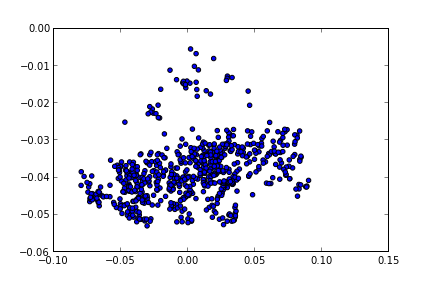
\includegraphics[height=6cm]{test_01.png}

\begin{minted}[fontsize=\footnotesize]{python}
clf = KMeans(n_clusters=2)
clf.fit(u)
labels_true = np.array(df['A16'])
labels_pred = clf.labels_
match = np.sum((labels_true == labels_pred).astype(int))
print float(match)/len(df)
\end{minted}

\begin{verbatim}
0.785604900459
\end{verbatim}









\end{document}
